\documentclass[12pt]{article}
\usepackage{polyglossia}
\usepackage[a4paper,hmargin=3.6cm]{geometry}
\usepackage{mathtools, amssymb, amsfonts}
\usepackage{amsthm}
\usepackage{fontspec}
\usepackage{titling}
\usepackage{float}
\usepackage{listings}
\usepackage{graphicx}
\usepackage{xcolor}
\usepackage{mdframed}
\usepackage{titling}
\usepackage{tikz}
\usepackage{listings}
\usepackage[hidelinks]{hyperref}
\usepackage{caption,subcaption}
\usepackage{tikz}
\usepackage[locale = FR, exponent-product = \cdot, inter-unit-product = .]{siunitx}
\usetikzlibrary{arrows,shapes,calc,angles,decorations.markings,patterns,decorations.pathmorphing}
\usepackage[shortlabels]{enumitem}
\usepackage{comment}

\setdefaultlanguage{french}
\frenchspacing

\newcommand{\RR}{\mathbb R}
\newcommand{\CC}{\mathbb C}
\newcommand{\QQ}{\mathbb Q}
\newcommand{\ZZ}{\mathbb Z}
\newcommand{\NN}{\mathbb N}
\newcommand{\KK}{\mathbb K}
\newcommand{\FF}{\mathbb F}
\newcommand{\LL}{\mathbb L}
\newcommand{\PP}{\mathbb P}
\newcommand{\EE}{\mathbb E}
\newcommand{\VV}{\mathbb V}

%%%
\theoremstyle{definition}

\newmdtheoremenv[%
	backgroundcolor=lightgray!10,
	linecolor=red!60!black,
	linewidth=2pt,
	topline=false,
	rightline=false,
	bottomline=false]{exer}{Exercice}


\pretitle{\begin{center}\LARGE
	\hrulefill\newline}
\title{\textsc{Tremplin: Séance 2}}
\posttitle{
\end{center}\vspace{-1em}
\hrulefill}
\date{\today}

\preauthor{}
\author{}
\postauthor{}

\begin{document}

\maketitle

\section*{Énoncés}

\begin{exer}
Un espion cherche à s'introduire dans les réseaux informatiques de l'entreprise \textsc{Thalès}, en travaillant avec un groupe de pirates basé à Hong Kong.

Il communique avec lui via une suite de messages encodés sur 2 bits (0 ou 1), mais il doit passer par une suite de $N$ terminaux << zombifiés >> différents. Pour un message donné, chaque ordinateur intermédiaire a une probabilité $q\in{]0,1[}$ de le modifier (0 est changé en 1 et réciproquement).
\begin{enumerate}
	\item Pour tout $n\in\NN$, on note $p_n$ la probabilité que le $n$-ème ordinateur renvoie le bon message. Déterminer une relation entre $p_{n+1}$ et $p_n$. 
	\item En déduire la probabilité que son collègue, sur le $N$-ème ordinateur, reçoive la bonne information.
	\item Que dire lorsque $N$ est très grand ? Pourquoi est-ce logique ?
\end{enumerate}
\end{exer}

\textit{Exercice de probabilité et de suites. Fait intervenir la notion de limite.}

\begin{exer}[Une introduction au théorème de Hahn-Banach]
On se place dans l'espace euclidien à trois dimensions $\RR^3$.
\begin{enumerate}
	\item Soient $A$ et $B$ deux points distincts de l'espace. Montrer qu'il existe un plan $(\mathcal{P})$ qui les sépare. On en explicitera l'équation cartésienne à partir des coordonnées des points $A$ et $B$ dans le repère orthonormé canonique $(0,\vec{\imath},\vec{\jmath},\vec k)$.
	\item On considère désormais deux droites disjointes $(\Delta_1)$ et $(\Delta_2)$. Montrer qu'il existe un plan qui les sépare.
	\item Même question avec deux sphères $(\mathcal S_1)$ et $(\mathcal S_2)$ de l'espace.
\end{enumerate}
\end{exer}

\textit{Exercice de géométrie analytique. Formalise une notion de séparation d'objets géométriques. Le théorème de Hahn-Banach est un des théorèmes fondamentaux de l'analyse fonctionnelle, branche des mathématiques qui étudie les fonctions prenant en argument... des fonctions !}

\begin{exer}[Il y a une infinité de nombre premiers]
	Démontrer qu'il y a une infinité de nombre premiers.
\end{exer}

\textit{Exercice d'arithmétique. Réintroduit la notion de nombre premier. Fait appel à des notions de logique, notamment le raisonnement par l'absurde.}


\begin{exer}[La mourre]
	Deux joueurs ont chacun une main dans le dos, avec un certain nombres de doigts dressés. Chacun annonce un nombre entre 0 et 10, puis ils présentent leur main cachée: celui qui a deviné le nombre total de doigts dressés gagne.
	
	Pourquoi certains totaux arrivent plus souvent que d'autres alors qu'on peut considérer que le nombre de doigts est aléatoire ?
\end{exer}

\textit{Exercice de dénombrement et probabilités.}

\begin{exer}[Marche aléatoire]
Jean-Michel est saoul et revient du bistrot. À chaque pas, il a une chance sur deux d'aller vers l'avant ou vers l'arrière. On suppose que sa maison est située à l'infini vers l'avant.
\begin{enumerate}
	\item Jean-Michel peut-il espérer rentrer chez lui ?
	\item La police est à la recherche de Jean-Michel, sachant qu'il a déjà effectué $t$ pas. Dans quelle zone autour du bar doit-elle chercher pour trouver Jean-Michel avec une certitude de 95\% ?
\end{enumerate}	

\end{exer}

\begin{figure}[!ht]
	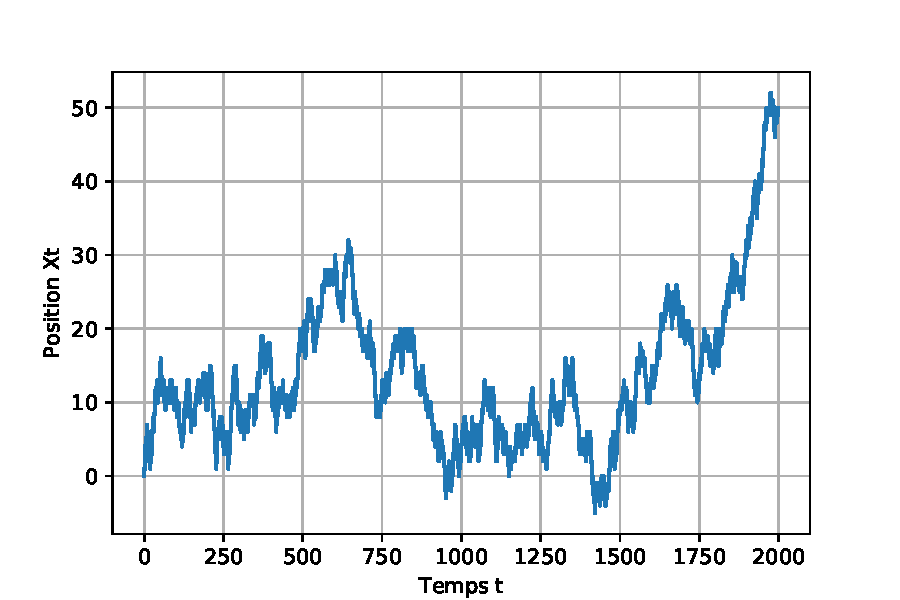
\includegraphics[width=0.9\textwidth]{../images/marcheJM.pdf}
	\caption{La marche de Jean-Michel}
\end{figure}

\textit{Il s'agit évidemment d'un exercice de probabilités sur les variables aléatoires. L'effort de formalisation porte surtout sur modéliser correctement le déplacement de l'ivrogne par une suite de variables de Rademacher.}

\clearpage

\section*{Correction}

\subsection*{Exercice 1}

1) Quand le message arrive dans l'ordinateur $N+1$, deux cas de figure se présentent: \begin{itemize}
\item soit le message sortant du $N$-ème ordinateur était le bon (avec probabilité $p_n$), dans lequel cas l'ordinateur suivant ne l'a pas modifié avec probabilité $1-q$
\item soit il était altéré (avec probabilité $1-p_n$) mais le terminal $N+1$ le ré-inverse pour redonner le bon avec probabilité $q$.
\end{itemize}
La probabilité que le message sortant du $N+1$-ème terminal soit correct est donc donné par
	\[ \tag{E}\label{recu}
	p_{n+1} = (1-q) p_n + q(1-p_n) = (1-2q)p_n + q. \]

2) En disant que le $0$-ème terminal est le poste de notre espion, la probabilité $p_0$ que le message en sortant soit correct est $1$. Le point fixe de la relation \eqref{recu} est $c = \frac 12$, est on en déduit la solution:
\[
p_n = \left(p_0 - \frac 12\right)(1-2q)^n + \frac 12 = \frac 12 (1-2q)^n + \frac 12.
\]

3) D'après la relation précédente, comme $-1 < 1-2q < 1$ quel que soit $q\in{]0,1[}$, on en déduit
\[
\lim_{n\to+\infty} p_n = \frac 12.
\]

La chose surprenante est bien évidemment le fait que la probabilité que le dernier ordinateur reçoive le bon est message est \textit{toujours} égale à $\frac 12$, quel que soit la probabilité $q$ que le message soit conservé à chaque fois !

\subsection*{Exercice 5}

On note $X_t$ la position de Jean-Michel à l'instant $t\in\NN$: c'est une variable aléatoire réelle discrète puisqu'il se déplace d'une unité à chaque instant.

Le déplacement entre les instants $t-1$ et $t$ est la variable aléatoire $\xi_t := X_t-X_{t-1}$. Cette variable aléatoire suit la loi de probabilité
\[
\PP(\xi_t = 1) = \PP(\xi_t = -1) = \frac{1}{2}. 
\]
Cette variable aléatoire finie admet pour espérance $\EE(\xi_t) = 0$, et les variables $(\xi_t)_{t\geq 0}$ suivent la même loi et sont indépendantes.

Un calcul simple montre que la position de Jean-Michel à l'instant $t$ est:
\[
X_t = \sum_{k=1}^t \xi_k,
\]
donc que son espérance mathématique, la position moyenne de Jean-Michel, est $\EE(X_t) = 0$.

\textit{La deuxième question, plus ambiguë, fait appel à quelques notions de statistiques, et peut servir d'introduction au théorème central limite pour faire le pont entre les probabilités et la maigre introduction aux statistiques en classe de Seconde.}

On cherche à donner un encadrement des positions successives $X_t$ de Jean-Michel qui soit vérifié dans la majeure partie des cas.

La variance de $X_t$ est donnée par la somme des variances des $(\xi_t)_{t\geq 0}$, qui valent $1$ :
\[
\VV(X_t) = \sum_{k=1}^t \VV(\xi_k) = t.
\]
L'écart-type est donc $\sigma(X_t) = \sqrt{t}$.

L'intuition suggère qu'après $t$ pas, la position de Jean-Michel serait bornée par l'écart-type $\sigma(X_t)$. On pourrait donc chercher une constante positive $c > 0$ telle que $|X_t| \leq c\sqrt{t}$ avec une << bonne certitude >> :
\[
\PP\left(|X_t|\leq c\sqrt t\right) =
\PP\left(-c\sqrt t \leq X_t \leq c\sqrt t\right) = 0,\!95.
\]

\textit{On présente ensuite aux élèves ce qu'est la loi normale et son usage en statistiques.}


Le théorème central limite dit que le $X_t/\sqrt{t}$ devient, en probabilité, proche d'une loi normale:
\[
\frac{X_t}{\sqrt{t}} \xrightarrow[t\to\infty]{\text{loi}} N
\]
où $N$ est une variable normale centrée réduite.

\textit{Il faut donc introduire la notion de convergence en loi d'une variable aléatoire.}
L'équation précédente donne pour $t$ grand $\PP(-c \leq N \leq c) = 0,\!95$ soit $2\Phi(c) - 1 = 0,\!95$ où $\Phi$ est la fonction de répartition de la loi normale centrée réduite. On obtient alors $c\approx 3,\!16$.

\textit{Pratique des probabilités; Effort de formalisation; Notion de convergence; Résultats classiques : Jean-Michel va passer une infinité de fois par tous les points du plan.}


\end{document}